\PassOptionsToPackage{table}{xcolor}
\documentclass[
    aspectratio=169
]{beamer}

\mode<presentation> {
\usetheme{Madrid}
\definecolor{Royalblue}{cmyk}{1, 0.72, 0, 0.38}
\usecolortheme[named=Royalblue]{structure}
\usefonttheme[onlymath]{serif}
}

\usepackage{graphicx}
\usepackage{booktabs}
\usepackage{caption}
\usepackage{multicol}
% xcolor already loaded by beamer with [table] option via PassOptionsToPackage

\setbeamertemplate{navigation symbols}{}
\setbeamertemplate{footline}
{
  \hbox{\begin{beamercolorbox}[wd=1\paperwidth,ht=2.25ex,dp=1ex,right]{framenumber}%
      \usebeamerfont{framenumber}{\color{black}{\insertframenumber{} / \inserttotalframenumber}}\hspace*{2ex}
    \end{beamercolorbox}}%
  \vskip0pt%
}

%----------------------------------------------------------------------------------------
%	TITLE PAGE
%----------------------------------------------------------------------------------------

\title[DT Fidelity]{{\textbf{Digital Twin Fidelity $\rightarrow$ Impact Analysis}}}

\subtitle{What Level of Detail Is Sufficient?}

\author{{\bf{{\large{Namhyun Kim}}}}}
\institute[ASU]
{
{\normalsize{Arizona State University}} \\
{\normalsize{School of Electrical, Computer and Energy Engineering (ECEE)}} \\
\medskip
}
\date{April 2026}

\begin{document}

\begin{frame}
\titlepage
\end{frame}

%------------------------------------------------
\begin{frame}{\textbf{Outline}}
\tableofcontents
\end{frame}

%------------------------------------------------
\section{Motivation \& Approach}
%------------------------------------------------

\begin{frame}{\textbf{Motivation \& Approach}}
\begin{block}{Core Question}
\centering
\large How does digital twin fidelity affect channel accuracy --- \\
and what level of detail is \textbf{sufficient}?
\end{block}

\vspace{0.3cm}
\begin{columns}[T]
\begin{column}{0.55\textwidth}
\textbf{Approach}:
\begin{enumerate}
    \item Build a high-fidelity \textbf{baseline} with Sionna RT.
    \item Systematically \textbf{degrade} along 4 axes.
    \item Measure \textbf{channel NMSE} at each level.
    \item Identify the \textbf{transition point} where accuracy breaks.
    \item Validate with \textbf{downstream ML tasks} (beam prediction, localization).
\end{enumerate}
\end{column}
\begin{column}{0.42\textwidth}
\begin{block}{4 Degradation Axes}
\begin{enumerate}
    \item \textbf{Geometry}: building position/shape
    \item \textbf{Material}: EM properties
    \item \textbf{Ray Tracing}: depth, ray count
    \item \textbf{Hardware}: antenna pattern, pol.
\end{enumerate}
\end{block}
\end{column}
\end{columns}
\end{frame}

%------------------------------------------------
\section{Experimental Setup}
%------------------------------------------------

\begin{frame}{\textbf{Evaluation Scenes}}
\vspace{-0.2cm}
\begin{columns}[T]
\begin{column}{0.48\textwidth}
\begin{center}
    \textbf{Simple Street Canyon} \\
    \vspace{0.2cm}
    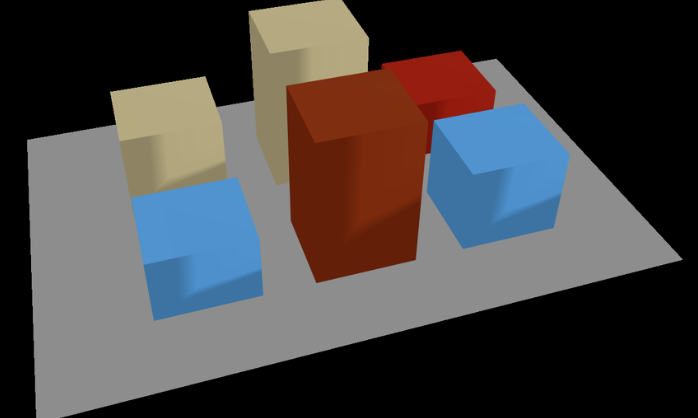
\includegraphics[width=0.85\linewidth,height=3.8cm,keepaspectratio]{simple_canyon.png}
\end{center}
\vspace{-0.1cm}
\begin{itemize}
    \item \footnotesize 2601 UEs ($51\times51$ grid, 0.8\,m spacing), 1 TX.
    \item \footnotesize Uniform canyon geometry --- clean multipath.
    \item \footnotesize \textbf{46/46 configs completed.}
\end{itemize}
\end{column}

\begin{column}{0.48\textwidth}
\begin{center}
    \textbf{Munich Urban Scene} \\
    \vspace{0.2cm}
    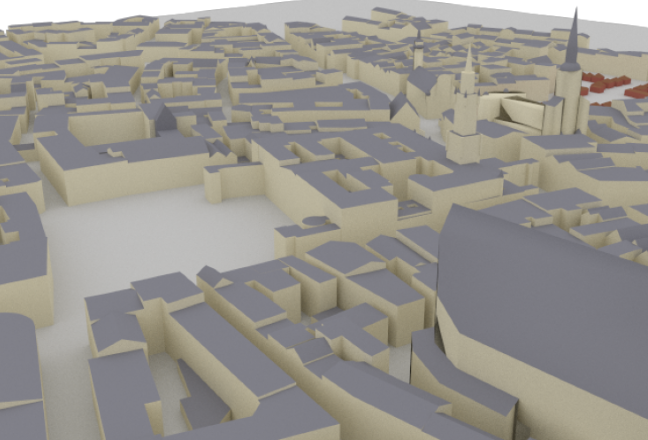
\includegraphics[width=0.85\linewidth,height=3.8cm,keepaspectratio]{munich.png}
\end{center}
\vspace{-0.1cm}
\begin{itemize}
    \item \footnotesize 2601 UEs, 332 buildings, diverse geometry.
    \item \footnotesize Realistic propagation with high scattering.
    \item \footnotesize \textbf{In progress} ($\sim$4\,h/config $\times$ 46 $=$ 164\,h).
\end{itemize}
\end{column}
\end{columns}
\end{frame}

%------------------------------------------------

\begin{frame}{\textbf{46 Degradation Configs Across 4 Axes}}
\vspace{-0.1cm}
\begin{columns}[T]
\begin{column}{0.48\textwidth}
\begin{block}{1. Geometry (12 configs)}
\begin{itemize}
    \item Position noise: 0.1, 0.5, 1, 2, 3, 4, 5, 7, 10\,m
    \item Height noise: 3\,m
    \item Building removal: small ($<$5\,m) or random 30\%
\end{itemize}
\end{block}
\begin{block}{2. Material (8 configs)}
\begin{itemize}
    \item Uniform override: concrete, glass, metal, wood, marble, brick
    \item Diffuse scattering on/off
\end{itemize}
\end{block}
\end{column}

\begin{column}{0.48\textwidth}
\begin{block}{3. Ray Tracing (20 configs)}
\begin{itemize}
    \item Reflection depth: 0, 1, 2, \ldots, 10
    \item Ray count: 1K, 5K, 10K, 20K, 50K, 100K, 200K, 500K
    \item Diffraction: 0 vs 1 event
\end{itemize}
\end{block}
\begin{block}{4. Hardware (5 configs)}
\begin{itemize}
    \item Pattern: TR38.901 vs Dipole vs Isotropic
    \item Spacing: $0.5\lambda$ vs $0.4\lambda$
    \item Polarization: V vs H
\end{itemize}
\end{block}
\end{column}
\end{columns}
\end{frame}

%------------------------------------------------
\section{Channel NMSE Results}
%------------------------------------------------

\begin{frame}{\textbf{Geometry: Sub-meter Accuracy Is Critical}}
\vspace{-0.2cm}
\begin{columns}[T]
\begin{column}{0.52\textwidth}
\begin{center}
    
\includegraphics[width=\linewidth,height=0.60\textheight,keepaspectratio]{../results/simple_street_canyon/geometry_sensitivity.png}
\end{center}
\end{column}
\begin{column}{0.45\textwidth}
\vspace{0.3cm}
\footnotesize
\begin{tabular}{rc}
\toprule
\textbf{Position Noise} & \textbf{NMSE (dB)} \\
\midrule
0.1\,m & $-8.2$ \\
0.5\,m & $-1.3$ \\
\rowcolor{red!15} 1\,m & $+10.6$ \\
\rowcolor{red!15} 2\,m & $+11.4$ \\
\rowcolor{red!30} 5\,m & $+12.0$ \\
\rowcolor{red!30} 10\,m & $+23.3$ \\
\bottomrule
\end{tabular}
\normalsize
\vspace{0.3cm}
\begin{block}{\footnotesize Transition Point}
\footnotesize $\leq$0.5\,m: usable ($-1.3$\,dB) \\
$\geq$1\,m: \textbf{broken} ($>+10$\,dB)
\end{block}
\end{column}
\end{columns}
\end{frame}

%------------------------------------------------

\begin{frame}{\textbf{Material: Surprisingly Low Impact}}
\vspace{-0.2cm}
\begin{columns}[T]
\begin{column}{0.52\textwidth}
\begin{center}
    
\includegraphics[width=\linewidth,height=0.60\textheight,keepaspectratio]{../results/simple_street_canyon/material_sensitivity.png}
\end{center}
\end{column}
\begin{column}{0.45\textwidth}
\vspace{0.3cm}
\footnotesize
\begin{tabular}{rc}
\toprule
\textbf{Material Config} & \textbf{NMSE (dB)} \\
\midrule
All concrete & $-1.50$ \\
All glass & $-0.73$ \\
All metal & $-1.47$ \\
All wood & $-1.69$ \\
All marble & $-1.57$ \\
All brick & $-1.46$ \\
No scattering & $-1.47$ \\
\bottomrule
\end{tabular}
\normalsize
\vspace{0.3cm}
\begin{block}{\footnotesize Key Finding}
\footnotesize Even replacing \textit{all} materials $\rightarrow$ only $\approx -1.5$\,dB NMSE. \\[3pt]
\textbf{Lowest priority} in simple canyon. \\
\textit{Pending: Munich validation.}
\end{block}
\end{column}
\end{columns}
\end{frame}

%------------------------------------------------

\begin{frame}{\textbf{Ray Tracing --- Reflection Depth: Diminishing Returns Above 5}}
\vspace{-0.2cm}
\begin{columns}[T]
\begin{column}{0.52\textwidth}
\begin{center}
    \includegraphics[width=\linewidth,height=0.60\textheight,keepaspectratio]{../results/simple_street_canyon/rt_depth_sensitivity.png}
\end{center}
\end{column}
\begin{column}{0.45\textwidth}
\vspace{0.3cm}
\footnotesize
\begin{tabular}{rc}
\toprule
\textbf{Max Depth} & \textbf{NMSE (dB)} \\
\midrule
0 (LoS only) & $-3.9$ \\
1 & $-8.2$ \\
2 & $-11.0$ \\
3 & $-10.8$ \\
\rowcolor{green!15} 5 & $-13.2$ \\
\rowcolor{green!15} 7 & $-12.1$ \\
10 (baseline) & ref \\
\bottomrule
\end{tabular}
\normalsize
\vspace{0.3cm}
\begin{block}{\footnotesize Transition Point}
\footnotesize Depth $\geq 3$: adequate ($< -10$\,dB) \\
Depth $\geq 5$: diminishing returns
\end{block}
\end{column}
\end{columns}
\end{frame}

%------------------------------------------------

\begin{frame}{\textbf{Ray Tracing --- Ray Count: 50K Is Enough}}
\vspace{-0.2cm}
\begin{columns}[T]
\begin{column}{0.52\textwidth}
\begin{center}
    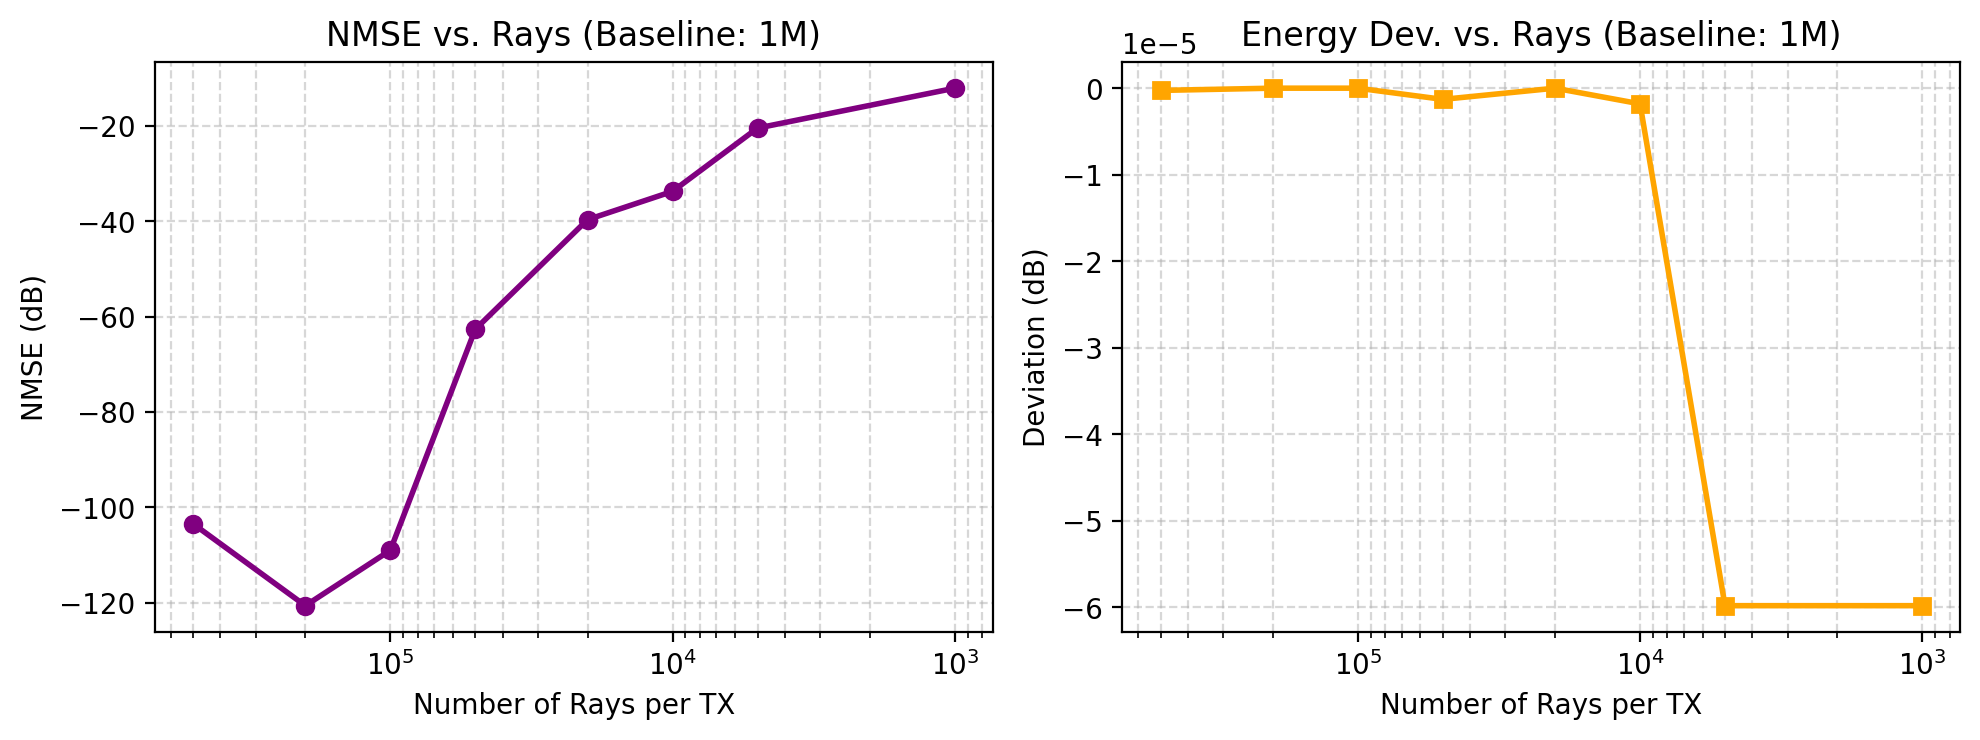
\includegraphics[width=\linewidth,height=0.60\textheight,keepaspectratio]{rt_ray_sensitivity.png}
\end{center}
\end{column}
\begin{column}{0.45\textwidth}
\vspace{0.3cm}
\footnotesize
\begin{tabular}{rc}
\toprule
\textbf{Ray Count} & \textbf{NMSE (dB)} \\
\midrule
1K & $-12.1$ \\
5K & $-20.5$ \\
\rowcolor{green!15} 50K & $-35.3$ \\
\rowcolor{green!15} 200K & $-40.6$ \\
1M (baseline) & ref \\
\bottomrule
\end{tabular}
\normalsize
\vspace{0.3cm}
\begin{block}{\footnotesize Transition Point}
\footnotesize $\geq$50K rays $\approx$ baseline quality \\
$\mathbf{20\times}$ speedup at negligible cost
\end{block}
\end{column}
\end{columns}
\end{frame}

%------------------------------------------------

\begin{frame}{\textbf{Hardware: Antenna Pattern Is Make-or-Break}}
\vspace{-0.2cm}
\begin{columns}[T]
\begin{column}{0.52\textwidth}
\begin{center}
    \includegraphics[width=\linewidth,height=0.55\textheight,keepaspectratio]{../results/simple_street_canyon/hardware_nmse.png}
\end{center}
\end{column}
\begin{column}{0.45\textwidth}
\vspace{0.3cm}
\footnotesize
\begin{tabular}{rc}
\toprule
\textbf{Hardware Config} & \textbf{NMSE (dB)} \\
\midrule
\rowcolor{red!30} Isotropic & $+21.7$ \\
\rowcolor{red!30} Dipole & $+23.5$ \\
\rowcolor{red!15} Polarization H & $+13.5$ \\
Spacing $0.4\lambda$ & $-8.4$ \\
TR38.901 (baseline) & ref \\
\bottomrule
\end{tabular}
\normalsize
\vspace{0.4cm}
\begin{block}{\footnotesize Key Finding}
\footnotesize Wrong pattern $\rightarrow$ NMSE $>+20$\,dB. \\
As damaging as 10\,m geometry noise. \\[3pt]
\textbf{Realistic pattern modeling is mandatory.}
\end{block}
\end{column}
\end{columns}
\end{frame}

%------------------------------------------------
\section{ML Task Validation}
%------------------------------------------------

\begin{frame}{\textbf{Step 6: Do Channel Thresholds Hold for ML Tasks?}}
\vspace{-0.1cm}
\begin{block}{Experiment Design}
\begin{itemize}
    \item \textbf{Train} beam prediction (position $\rightarrow$ beam) and localization (channel $\rightarrow$ position) on \textit{degraded} DT data.
    \item \textbf{Test} on \textit{baseline} data $=$ simulated reality.
    \item Question: At what fidelity does ML task performance collapse?
\end{itemize}
\end{block}
\vspace{-0.1cm}
\begin{center}
    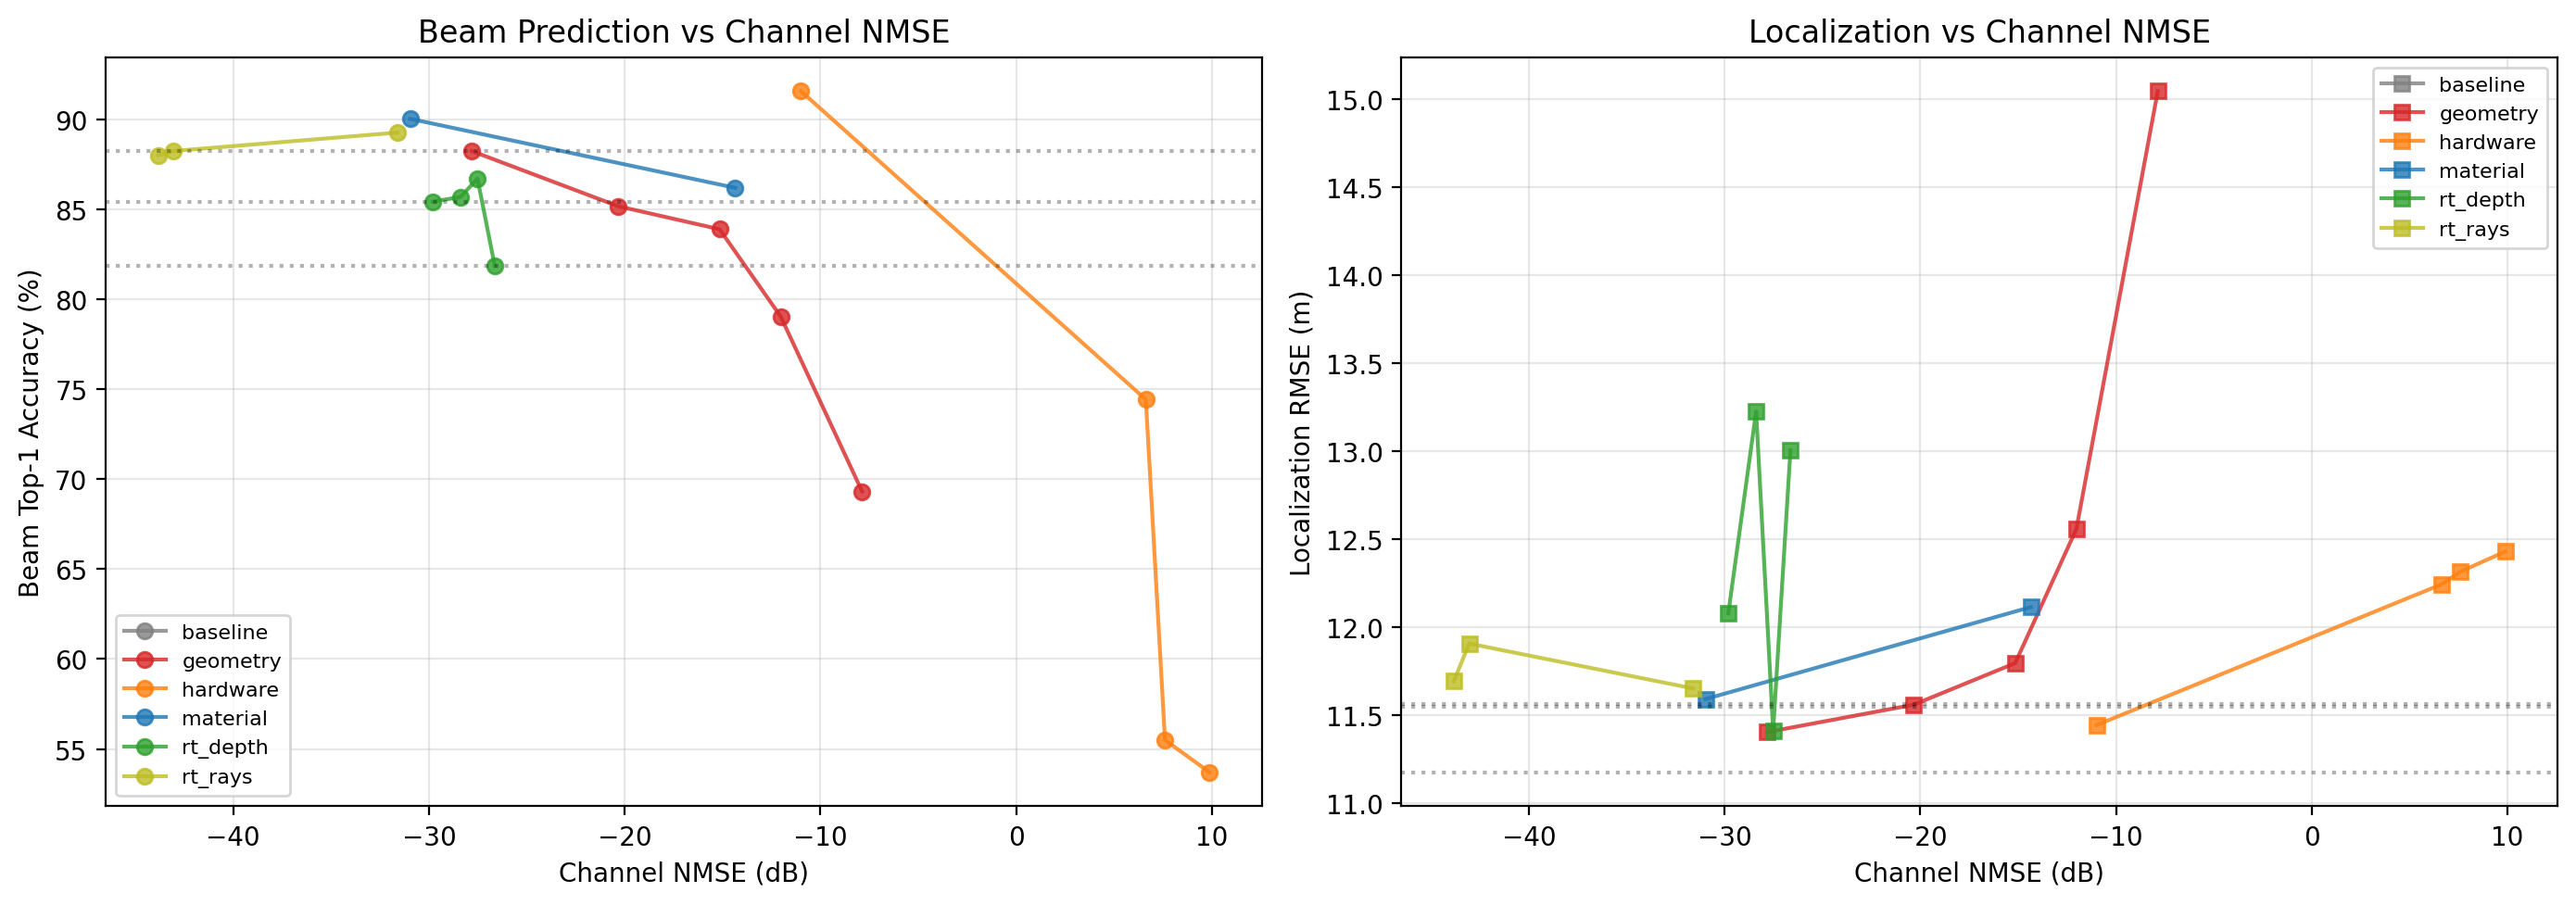
\includegraphics[width=0.92\linewidth,height=0.45\textheight,keepaspectratio]{ml_task_vs_nmse.png}
\end{center}
\vspace{-0.2cm}
\footnotesize
\textbf{Key insight}: ML tasks are more tolerant than raw NMSE --- geometry up to 2\,m and RT depth=2 still yield $>$79\% beam accuracy, while their channel NMSE is already degraded.
\end{frame}

%------------------------------------------------

\begin{frame}{\textbf{ML Results: Geometry --- Gradual Degradation}}
\vspace{-0.1cm}
\begin{center}
    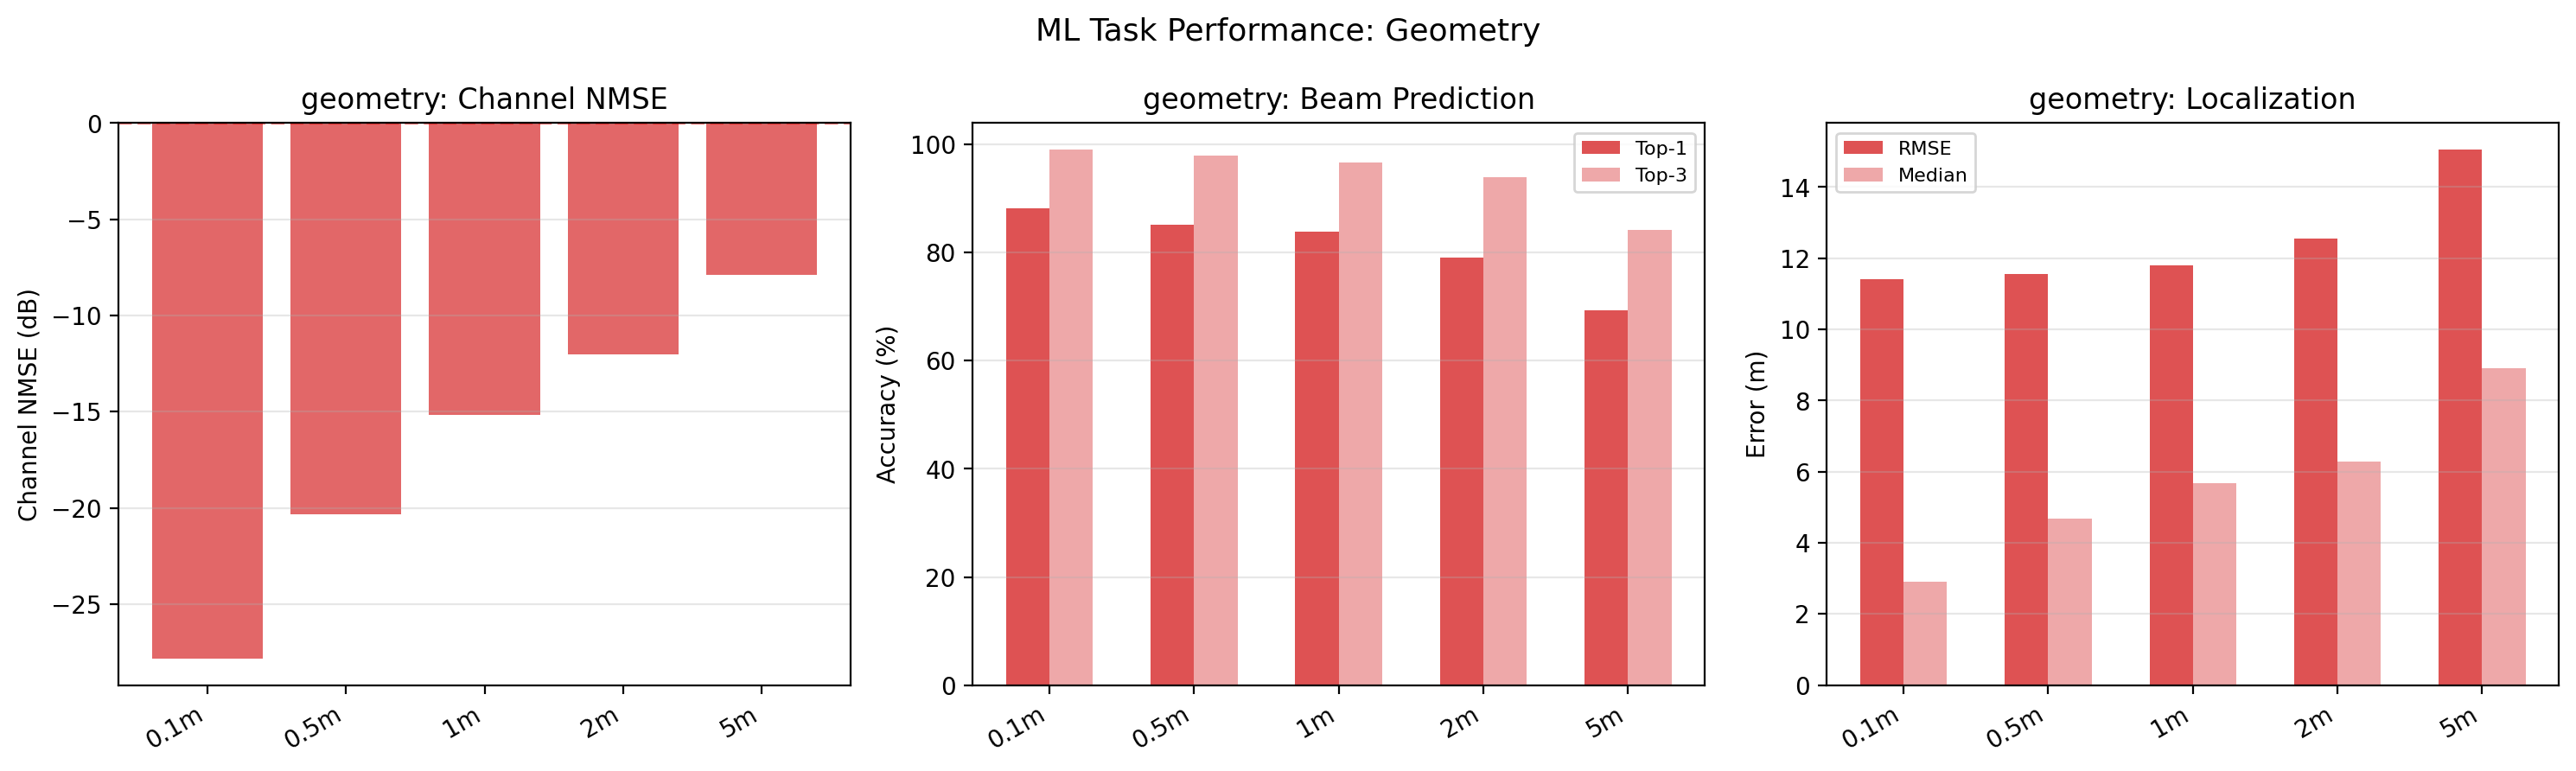
\includegraphics[width=0.92\linewidth,height=0.45\textheight,keepaspectratio]{ml_geometry_detail.png}
\end{center}
\vspace{-0.2cm}
\footnotesize
\begin{columns}[T]
\begin{column}{0.48\textwidth}
\begin{tabular}{rccc}
\toprule
\textbf{Noise} & \textbf{NMSE} & \textbf{Beam T1} & \textbf{Gain} \\
\midrule
0.1\,m & $-8.2$ & 88.2\% & 94.7\% \\
0.5\,m & $-1.3$ & 85.2\% & 95.5\% \\
1\,m & $+10.6$ & 83.9\% & 91.3\% \\
2\,m & $+11.4$ & 79.0\% & 91.8\% \\
\rowcolor{red!15} 5\,m & $+12.0$ & 69.3\% & 82.1\% \\
\bottomrule
\end{tabular}
\end{column}
\begin{column}{0.48\textwidth}
\begin{block}{\footnotesize Finding}
\footnotesize
\begin{itemize}
    \item Channel NMSE breaks at 1\,m ($+10.6$\,dB).
    \item But beam accuracy still 84\% at 1\,m.
    \item ML threshold is $\sim$2--5\,m, \textbf{more tolerant} than channel NMSE.
\end{itemize}
\end{block}
\end{column}
\end{columns}
\end{frame}

%------------------------------------------------

\begin{frame}{\textbf{ML Results: Hardware --- Pattern Errors Are Fatal}}
\vspace{-0.1cm}
\begin{center}
    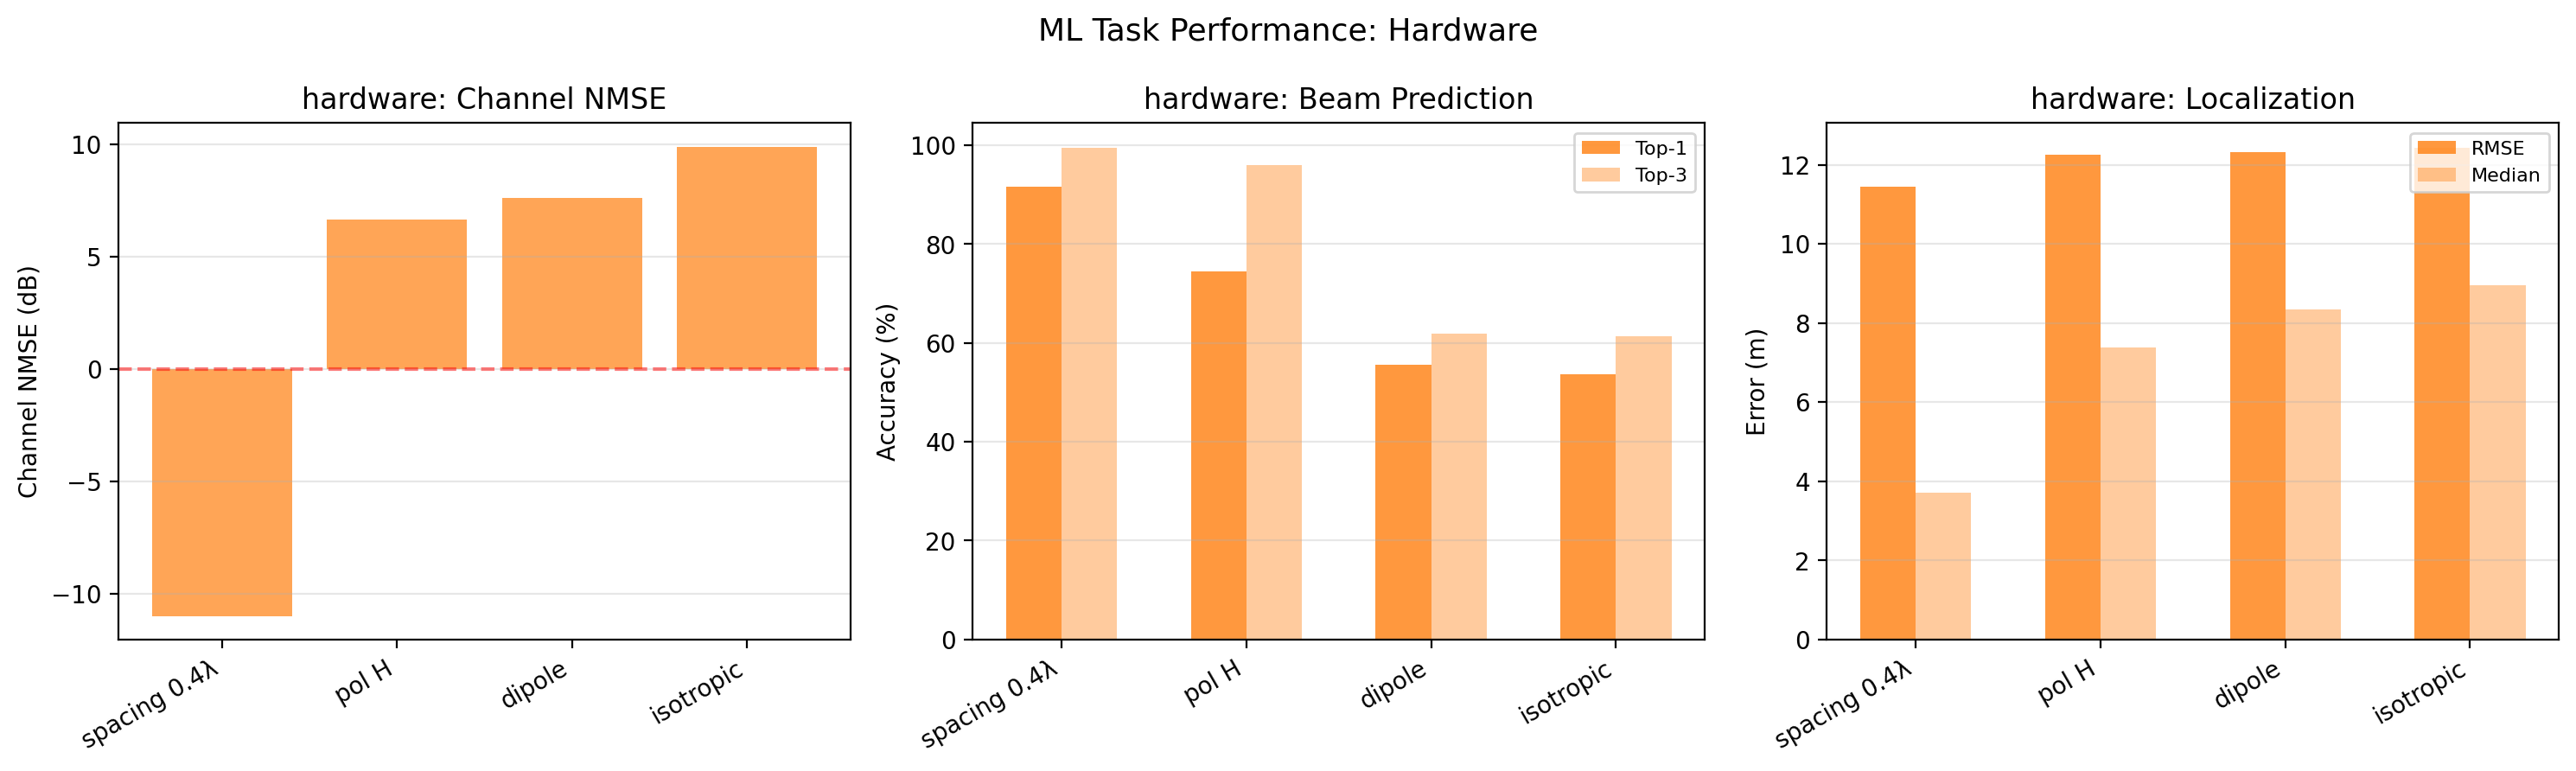
\includegraphics[width=0.92\linewidth,height=0.45\textheight,keepaspectratio]{ml_hardware_detail.png}
\end{center}
\vspace{-0.2cm}
\footnotesize
\begin{columns}[T]
\begin{column}{0.48\textwidth}
\begin{tabular}{rccc}
\toprule
\textbf{Config} & \textbf{NMSE} & \textbf{Beam T1} & \textbf{Gain} \\
\midrule
Spacing & $-8.4$ & 91.6\% & 96.6\% \\
Pol H & $+13.5$ & 74.4\% & 88.4\% \\
\rowcolor{red!30} Dipole & $+23.5$ & 55.5\% & 32.8\% \\
\rowcolor{red!30} Isotropic & $+21.7$ & 53.7\% & 29.6\% \\
\bottomrule
\end{tabular}
\end{column}
\begin{column}{0.48\textwidth}
\begin{block}{\footnotesize Finding}
\footnotesize
\begin{itemize}
    \item Dipole/Isotropic: beam gain $\approx 30\%$.
    \item Model picks beams that capture only 1/3 of optimal power.
    \item \textbf{Pattern fidelity is non-negotiable} for both NMSE and ML.
\end{itemize}
\end{block}
\end{column}
\end{columns}
\end{frame}

%------------------------------------------------

\begin{frame}{\textbf{ML Results: Material \& Ray Tracing --- Robust}}
\vspace{-0.1cm}
\footnotesize
\begin{columns}[T]
\begin{column}{0.48\textwidth}
\begin{block}{Material}
\begin{tabular}{rccc}
\toprule
\textbf{Config} & \textbf{NMSE} & \textbf{Beam T1} & \textbf{Gain} \\
\midrule
All concrete & $-1.5$ & 86.2\% & 96.0\% \\
All metal & $-1.5$ & 90.0\% & 95.7\% \\
\midrule
\textit{Baseline} & \textit{ref} & \textit{88.2\%} & \textit{97.4\%} \\
\bottomrule
\end{tabular}
\vspace{0.2cm}
\footnotesize Material changes have \textbf{no measurable ML impact}. Uniform material assignment is acceptable.
\end{block}
\end{column}
\begin{column}{0.48\textwidth}
\begin{block}{Ray Tracing}
\begin{tabular}{rccc}
\toprule
\textbf{Config} & \textbf{NMSE} & \textbf{Beam T1} & \textbf{Gain} \\
\midrule
Depth=2 & $-11.0$ & 81.8\% & 89.7\% \\
Depth=3 & $-10.8$ & 85.7\% & 93.8\% \\
Depth=5 & $-13.2$ & 85.4\% & 93.1\% \\
Depth=7 & $-12.1$ & 86.7\% & 95.2\% \\
\midrule
5K rays & $-20.5$ & 88.2\% & 94.3\% \\
50K rays & $-35.3$ & 88.0\% & 94.1\% \\
\midrule
\textit{Baseline} & \textit{ref} & \textit{82--88\%} & \textit{93--97\%} \\
\bottomrule
\end{tabular}
\vspace{0.1cm}
\footnotesize Depth $\geq 3$: beam accuracy within 3\% of baseline. \\ Ray count: even 5K rays has \textbf{no ML impact}.
\end{block}
\end{column}
\end{columns}
\end{frame}

%------------------------------------------------
\section{Sufficient Detail: Combined Thresholds}
%------------------------------------------------

\begin{frame}{\textbf{Answer: What Level of Detail Is Sufficient?}}
\vspace{-0.3cm}
\begin{center}
\footnotesize
\begin{tabular}{lccccc}
\toprule
 & & \multicolumn{2}{c}{\textbf{Channel}} & \multicolumn{2}{c}{\textbf{ML Task}} \\
\cmidrule(lr){3-4} \cmidrule(lr){5-6}
\textbf{Axis} & \textbf{Threshold} & \textbf{NMSE} & \textbf{OK?} & \textbf{Beam} & \textbf{OK?} \\
\midrule
\textbf{Geometry} $\leq 0.5$\,m & NMSE thr. & $-1.3$\,dB & \checkmark & 85\% & \checkmark \\
\textbf{Geometry} $\leq 2$\,m & ML thr. & $+11.4$\,dB & $\times$ & 79\% & \checkmark \\
\textbf{Material} & Any & $-1.5$\,dB & \checkmark & 86--90\% & \checkmark \\
\textbf{RT Depth} $\geq 3$ & Both & $-10.8$\,dB & \checkmark & 86\% & \checkmark \\
\textbf{RT Rays} $\geq 5$K & Both & $-20.5$\,dB & \checkmark & 88\% & \checkmark \\
\textbf{HW Pattern} & TR38.901 & ref & \checkmark & 86\% & \checkmark \\
\textbf{HW Pattern} & Dipole/Iso & $+22$\,dB & $\times$ & 54\% & $\times$ \\
\textbf{HW Pol.} & Must match & $+13.5$\,dB & $\times$ & 74\% & $\sim$ \\
\textbf{HW Spacing} & $\pm 0.1\lambda$ & $-8.4$\,dB & \checkmark & 92\% & \checkmark \\
\bottomrule
\end{tabular}
\end{center}

\vspace{0.05cm}
\begin{block}{Key Takeaway}
\footnotesize
\begin{itemize}\setlength{\itemsep}{1pt}
    \item \textbf{ML tasks are more tolerant than channel NMSE}: geometry 2\,m still gives 79\% beam accuracy despite $+11$\,dB NMSE.
    \item \textbf{Exception --- hardware}: antenna pattern errors break \textit{both} channel and ML equally.
    \item \textbf{Biggest speedup opportunity}: ray count can be reduced $200\times$ (1M $\rightarrow$ 5K) with zero ML impact.
\end{itemize}
\end{block}
\end{frame}

%------------------------------------------------
\section{Real-World Validation}
%------------------------------------------------

\begin{frame}{\textbf{Real-World Validation: Setup}}
\vspace{-0.2cm}
\footnotesize
\begin{columns}[T]
\begin{column}{0.48\textwidth}
\begin{block}{DICHASUS Dataset (dcxx)}
\begin{itemize}\setlength{\itemsep}{1pt}
    \item Real indoor channel measurements at 3.438\,GHz, 50\,MHz bandwidth.
    \item 64 distributed antennas (2 arrays of 4$\times$8) in a hallway.
    \item 1024 OFDM subcarriers, tachymeter ground-truth positions.
    \item Source: Univ.\ Stuttgart, used in NVlabs' diff-RT calibration.
\end{itemize}
\end{block}
\end{column}
\begin{column}{0.48\textwidth}
\begin{block}{Simplified 3D Scene}
\begin{itemize}\setlength{\itemsep}{1pt}
    \item \texttt{inue\_simple}: only 3 objects --- walls, floor, ceiling.
    \item ITU material models (concrete, plasterboard, ceiling board).
    \item No furniture, pillars, doors, columns, or other scatterers.
    \item \textbf{Analogous to severe geometry degradation} in our framework.
\end{itemize}
\end{block}
\begin{block}{Experiment}
\begin{itemize}\setlength{\itemsep}{1pt}
    \item Sionna 2.0 PathSolver: max\_depth=5, 500K samples.
    \item 40 measurement positions, compare RT vs measured CSI.
\end{itemize}
\end{block}
\end{column}
\end{columns}
\end{frame}

%------------------------------------------------

\begin{frame}{\textbf{Real-World Validation: Results}}
\vspace{-0.2cm}
\begin{center}
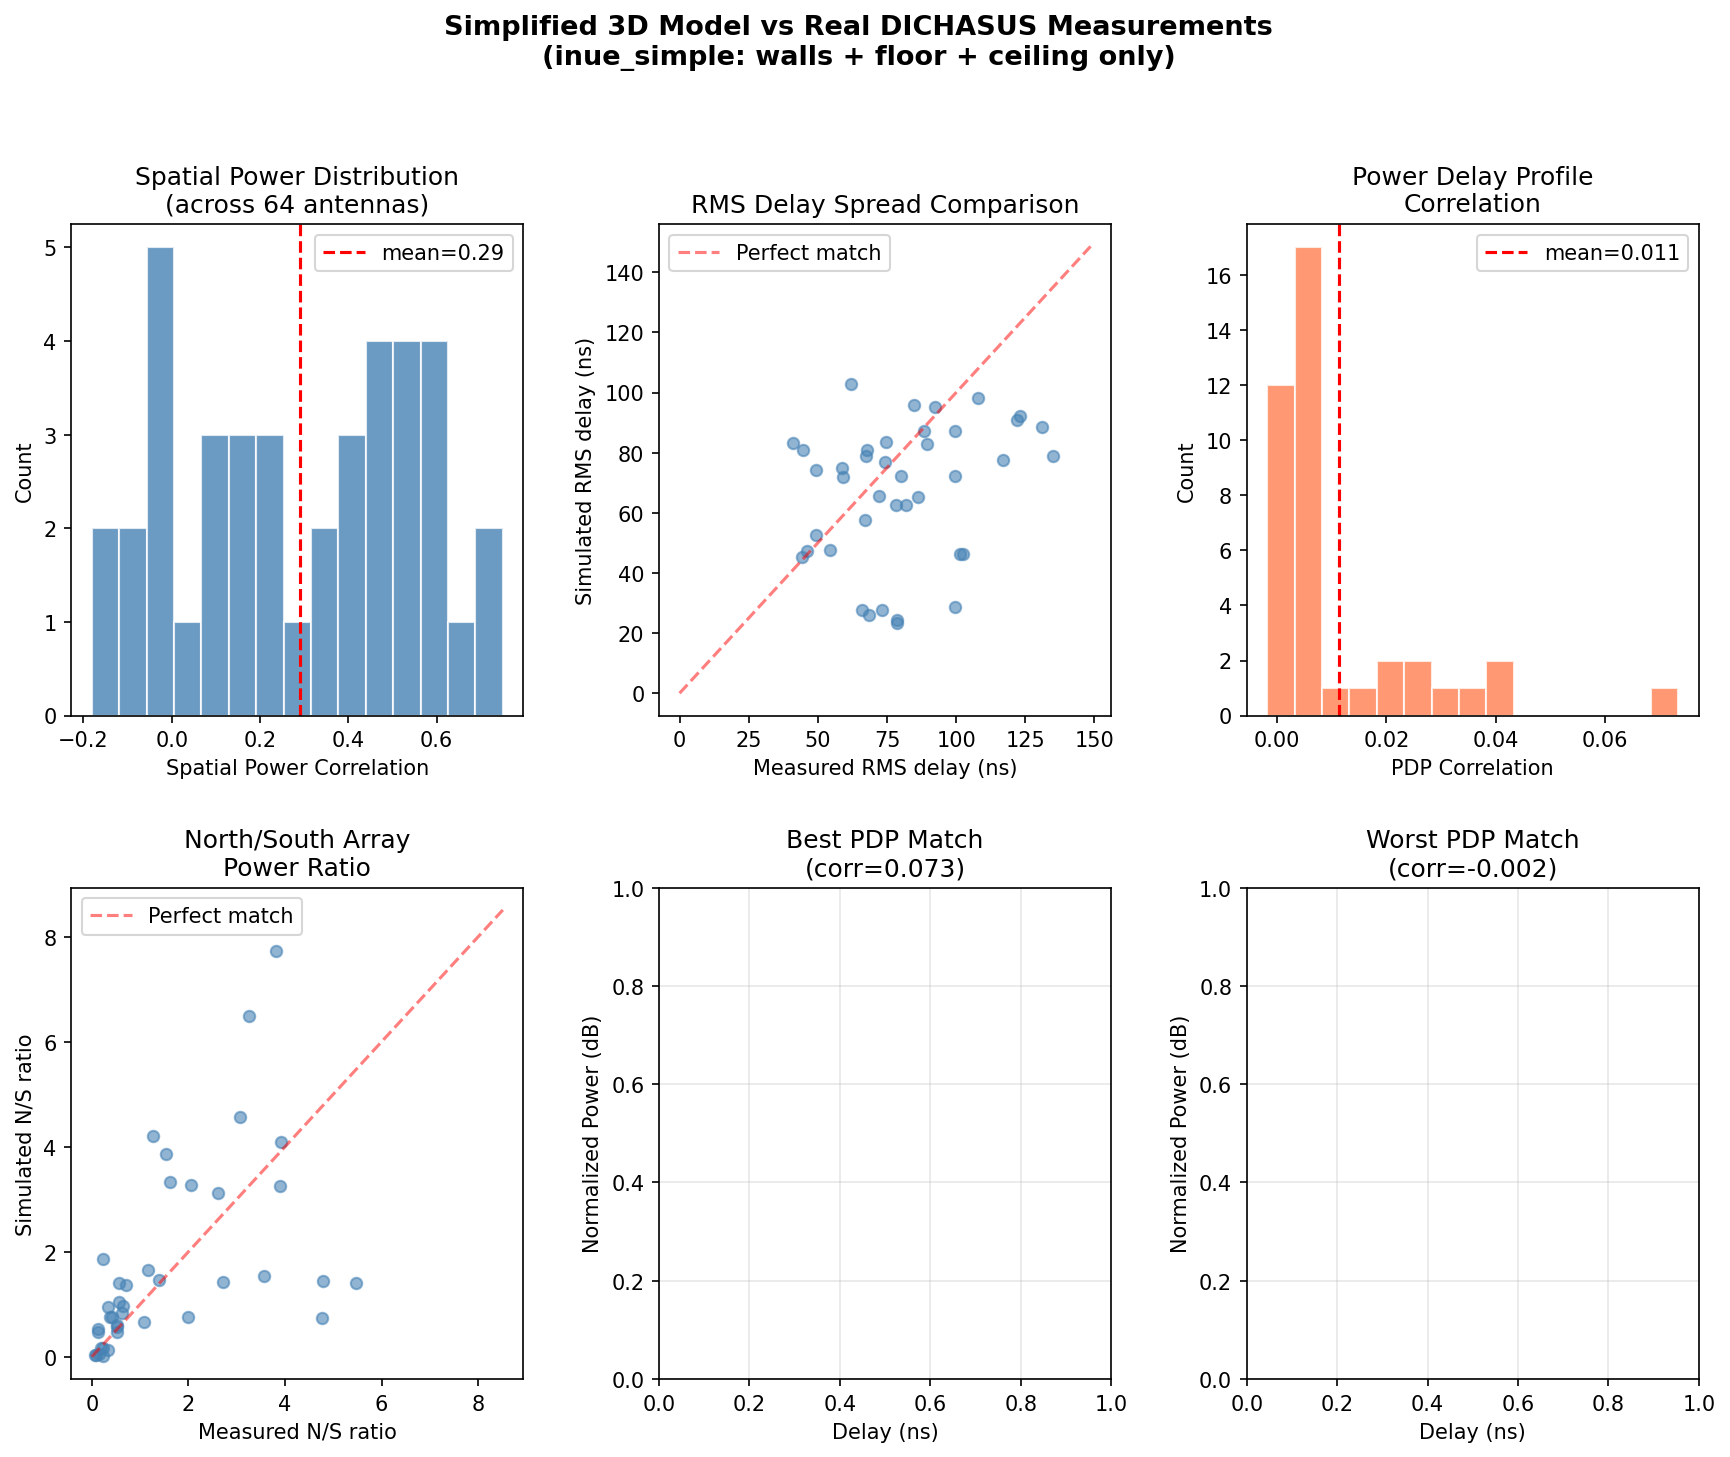
\includegraphics[width=0.92\linewidth,height=0.82\textheight,keepaspectratio]{real_world_validation.png}
\end{center}
\end{frame}

%------------------------------------------------

\begin{frame}{\textbf{Real-World Validation: Key Findings}}
\vspace{-0.3cm}
\begin{center}
\footnotesize
\begin{tabular}{l c c l}
\toprule
\textbf{Metric} & \textbf{Value} & \textbf{Interpretation} & \textbf{Framework Prediction} \\
\midrule
Spatial power corr. & $r = 0.29$ & Partial & Large-scale OK \\
RMS delay error & 25\,ns avg & Approximate & Envelope OK \\
PDP correlation & $r = 0.01$ & \cellcolor{red!15}None & \cellcolor{red!15}Multipath fails \\
CFR correlation & $r = 0.05$ & \cellcolor{red!15}None & \cellcolor{red!15}Channel fails \\
Scaled NMSE & $\approx 0$\,dB & \cellcolor{red!15}Uncorrelated & \cellcolor{red!15}Expected \\
\bottomrule
\end{tabular}
\end{center}

\vspace{0.05cm}
\begin{block}{Confirmation of Fidelity Framework}
\footnotesize
\begin{itemize}\setlength{\itemsep}{1pt}
    \item \textbf{Geometry dominates}: simplified scene (walls only) captures large-scale power distribution but completely misses multipath structure --- exactly as predicted by our synthetic experiments.
    \item \textbf{Consistent with Canyon results}: geometry degradation $>$2\,m causes NMSE $>$+10\,dB; the simplified INUE scene omits all interior objects (equivalent to $\gg$5\,m error).
    \item \textbf{Next}: add detailed geometry from full 3D model to improve match, then apply degradation framework.
\end{itemize}
\end{block}
\end{frame}

%------------------------------------------------

\begin{frame}{\textbf{Power Delay Profile: Simulated vs Measured}}
\vspace{-0.2cm}
\begin{center}
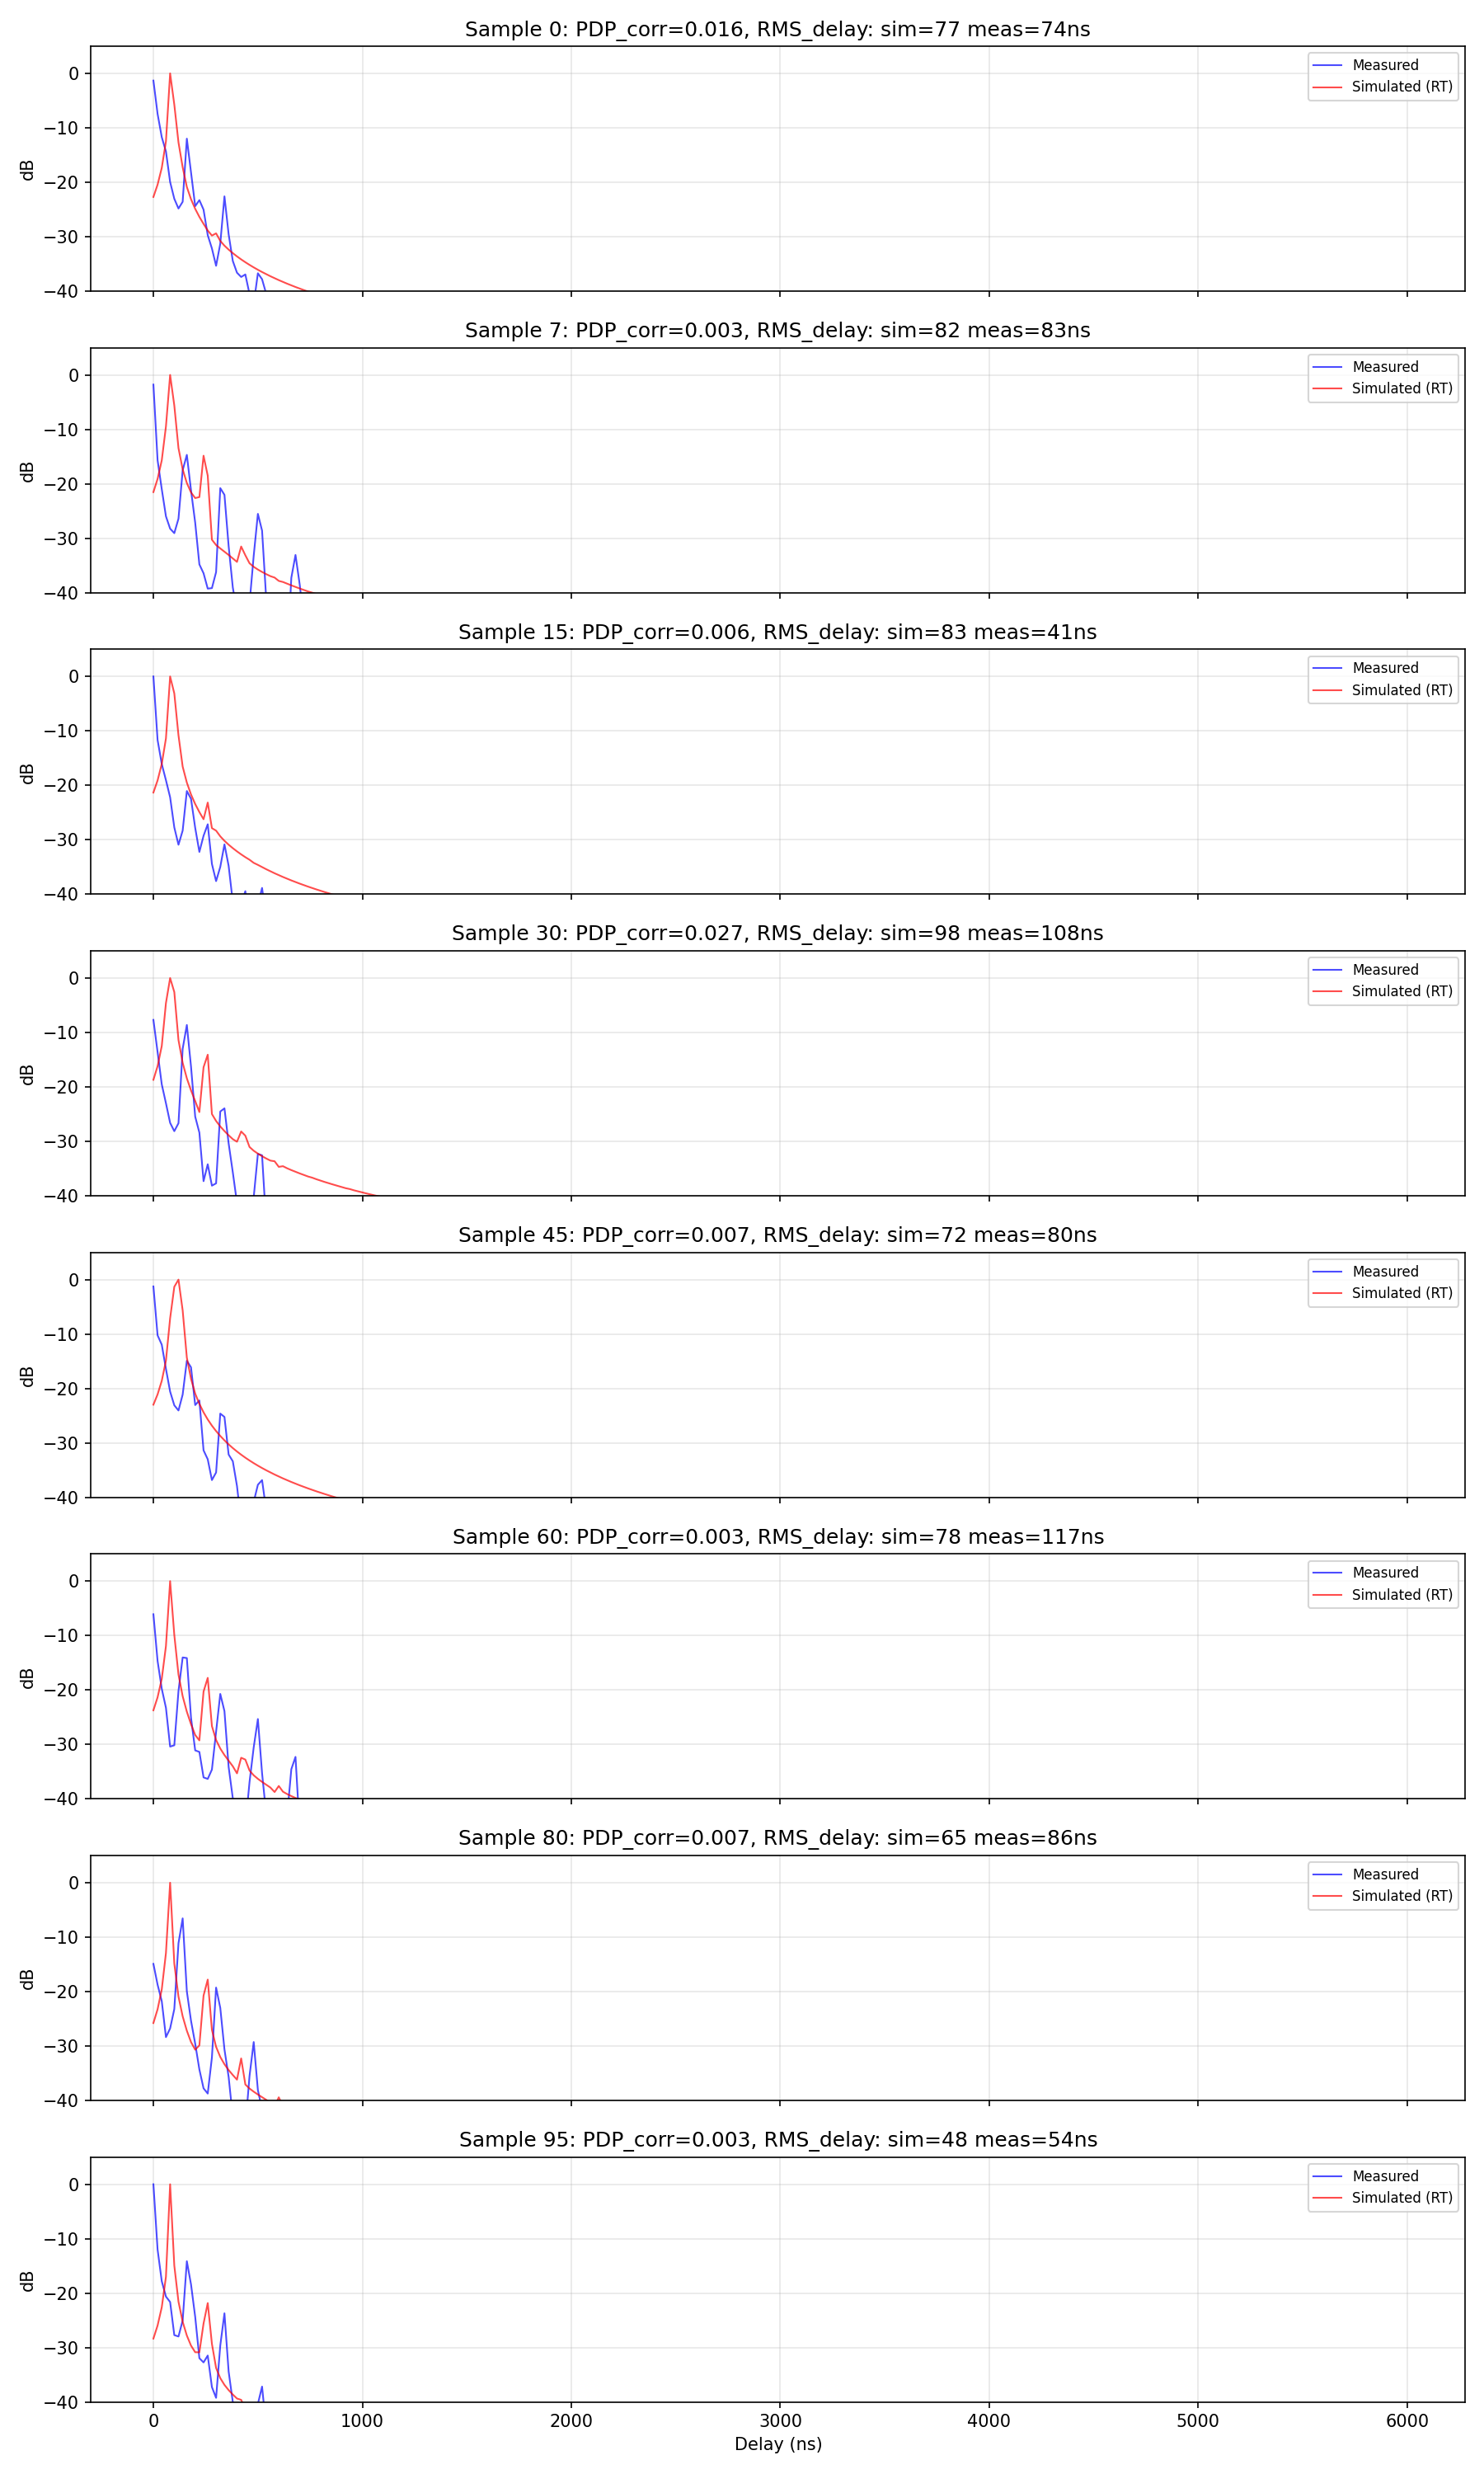
\includegraphics[width=0.72\linewidth,height=0.72\textheight,keepaspectratio]{pdp_comparison.png}
\end{center}
\vspace{-0.3cm}
\footnotesize
Simplified scene captures general delay envelope but misses detailed multipath taps. Measured PDPs show richer scattering from objects absent in the 3-surface model.
\end{frame}

%------------------------------------------------
\section{Remaining Work}
%------------------------------------------------

\begin{frame}{\textbf{Remaining Work}}
\begin{columns}[T]
\begin{column}{0.48\textwidth}
\begin{block}{Completed}
\begin{itemize}
    \item[\checkmark] Canyon: 46 configs, NMSE + ML analysis.
    \item[\checkmark] Per-axis threshold table (channel + ML).
    \item[\checkmark] Real-world validation with DICHASUS.
\end{itemize}
\end{block}
\begin{block}{In Progress}
\begin{itemize}
    \item Munich 50$\times$50: 46 configs ($\sim$4\,h/config, 164\,h total).
    \item Detailed INUE scene from full .blend model.
\end{itemize}
\end{block}
\end{column}

\begin{column}{0.48\textwidth}
\begin{block}{Next Steps}
\begin{itemize}
    \item Build detailed 3D model $\rightarrow$ show improved NMSE.
    \item Apply fidelity degradation to INUE scene.
    \item \textbf{Key question}: Can calibrated RT on detailed scene achieve NMSE $< -10$\,dB vs real measurements?
\end{itemize}
\end{block}
\begin{block}{Cross-Scene Validation}
\begin{itemize}
    \item Repeat analysis on Munich.
    \item Does material fidelity matter more in complex urban geometry?
\end{itemize}
\end{block}
\end{column}
\end{columns}
\end{frame}

%------------------------------------------------

\begin{frame}
\begin{center}
    \Large Questions?
\end{center}
\end{frame}

\end{document}
